\documentclass{classrep}
\usepackage[utf8]{inputenc}
\frenchspacing

\usepackage{graphicx}
\usepackage[usenames,dvipsnames]{color}
\usepackage[hidelinks]{hyperref}
\usepackage{lmodern}
\usepackage{placeins}
\usepackage{url}
\usepackage{amsmath, amssymb, mathtools}
\usepackage{listings}
\usepackage{fancyhdr, lastpage}

\pagestyle{fancyplain}
\fancyhf{}
\renewcommand{\headrulewidth}{0pt}
\cfoot{\thepage\ / \pageref*{LastPage}}

%--------------------------------------------------------------------------------------%
\studycycle{Informatyka stosowana, studia dzienne, II st.}
\coursesemester{II}

\coursename{Analiza danych złożonych}
\courseyear{2021/2022}

\courseteacher{dr hab inż. Agnieszka Duraj}
\coursegroup{środa, 11:00}

\author{%
    \studentinfo[239671@edu.p.lodz.pl]{Jan Karwowski}{239671}\\
    \studentinfo[239676@edu.p.lodz.pl]{Kamil Kowalewski}{239676}\\
}

\title{Zadanie 4.: Metody grawitacyjne i kątowe}

\begin{document}
    \maketitle
    \thispagestyle{fancyplain}

    \tableofcontents
    \newpage

    \section{Cel} {
        Celem zadania jest dokonanie analizy danych dla trzech zbiorów danych przy
        pomocy wybranych algorytmów należących do grupy metody grawitacyjnych i kątowych.
    }

    \section{Zbiory danych} {
        Do przeprowadznia badań w tym zadaniu zostały wykorzystane trzy zbiory danych,
        dwa z nich są zbiorami naturalnymi natomiast jeden z nich jest sztucznie
        wygenerowany.

        Zbiór wygenerowany sztucznie został utworzony poprzez wykorzystanie funkcji
        \textit{generate\_data}, która jest wbudowana w bibliotekę
        \textit{PyOD}\cite{pyod}. Zbiór ten ma 2 wymiary natomiast procent wyjątków
        został ustawiony na wartość równą \textit{10\%}.

        Drugi i trzeci zbiór danych pochodzą z serwisu \emph{Outlier Detection DataSets}
        \cite{odds}, który zawiera kilkadziesiąt przykładowych zbiorów
        danych, dostosowanych do zadania wyszukiwania wyjątków. Zbiory te są już
        znormalizowane i oczyszczone, każdy przykład w każdym zbiorze jest oznaczony
        jedną z dwóch klas: wyjątek lub nie wyjątek. Wybranymi zbiorami są ,,http''
        oraz ,,mammography''.

        Zbiór ,,http'' zawiera 3 kolumny i oryginalnie ponad 500 tys. wierszy, z czego
        ok. 0.4\% stanowią wyjątki. Zbiór ten na potrzebny niniejszego zadania został
        ograniczony do ok 1\% próbek, przy czym proporcja wyjątków została zachowana.
        Zbiór ten zawiera informacje o zapytaniach HTTP.

        Zbiór ,,mammography'' zawiera 6 kolumn i ponad 11 tys. wierszy, z czego ok. 2\%
        stanowią wyjątki. Zbiór ten dotyczy wyników badania mammograficznego i
        wyjątkami są przypadki zdiagnozowane jako chore, których jest stosunkowo mało
        do przypadków zdrowych, przez co zbiór ten został dostosowany do zadania
        rozpoznawania wyjątków, chociaż oryginalnie dotyczy zadania klasyfikacji.
    }

    \section{Implementacja} {
        Program został napisany w języku Python z wykorzystaniem biblioteki
        \textit{PyOD}\cite{pyod} aby skorzystać z gotowych implementacji algorytmów
        Wybranym algorytmem jest:
        \begin{itemize}
            \item FastABOD (ang. Angle-Based Outlier Detection)
        \end{itemize}

        Samo uruchomienie programu dokonywane jest poprzez komendę
        \textit{python main.py}. W jego czasie wykonywane są wszystkie eksperymenty
        zaplanowane przez autorów.
    }

    \section{Opis algorytmu FastABOD} {
        Algorytm ABOD to algorytm znajdujący wyjątki w zbiorze danych na
        podstawie kąta między danym punktem (elementem zbioru danych) a
        parami innych punktów. Algorytm działa na zasadzie podobnej do LOF
        i przypisuje każdemu elementowi ze zbioru danych pewną wartość
        (score), która oznacza jak bardzo dany punkt jest wyjątkiem. W
        przeciwieństwie jednak do algorytmu LOF podstawa działania tego
        rankingu w algorytmie ABOD nie jest odległość między punktami ale
        kąty pomiędzy nimi. Metoda ta ma według autorów stanowić
        rozwiązania problemu ,,przekleństwa wymiarowości'', który polega na
        tym, że w zbiorach danych o bardzo dużej liczbie wymiarów wszystkie
        punkty są w podobnych odległościach do siebie. Sama wartość (score)
        dla danego punktu wynika z wariancji kątów między tym punktem, a
        parami pozostałych punktów w zbiorze. Intuicyjnie dla punktów
        znajdujących się w obrębie klastra wariancja ta będzie duża,
        natomiast dla punktów znajdujących się daleko od najbliższego
        zgrupowania, kąty te zawsze będą małe i wariancja również. Ze
        względu na dużą złożoność obliczeniową tej metody $O(n)=n^3$
        autorzy zaproponowali prostą modyfikację, polegającą na
        uwzględnieniu jedynie $n$ najbliższych sąsiadów - jest to algorytm
        FastABOD.
    }

    \section{Eksperymenty} {

        We wszystkich eksperymentach dla wszystkich trzech algorytmów
        parametr ,,n\_neighbors'' (n najbliższych sąsiadów) został
        ustawiony na wartość $50$.

        \begin{figure}[!htbp]
            \centering
            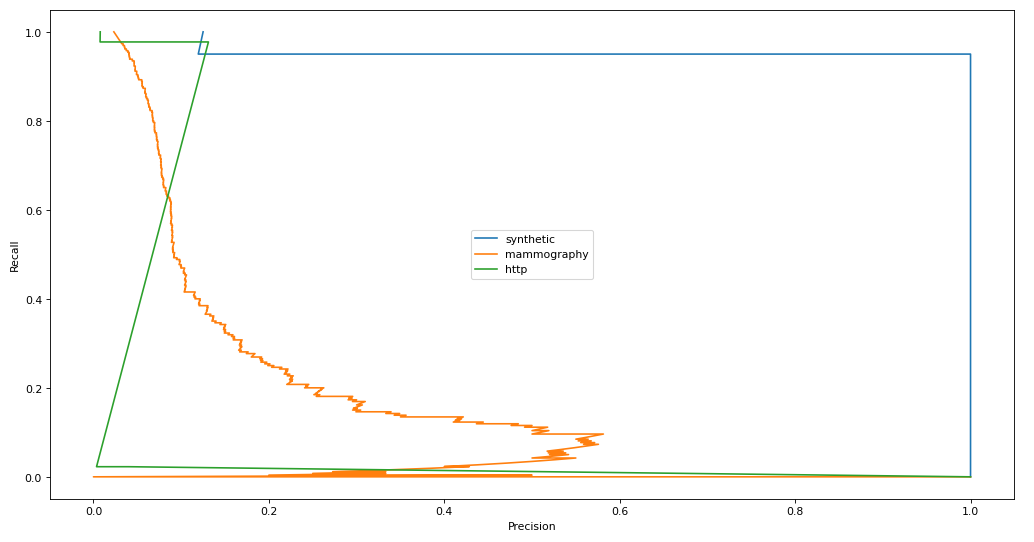
\includegraphics[width=\textwidth]{img/recall_precision_abod.png}
            \caption
            {Wykres recall od precision dla metody ABOD dla 3 zbiorów danych}
            \label{fig:abod}
        \end{figure}

        \begin{figure}[!htbp]
            \centering
            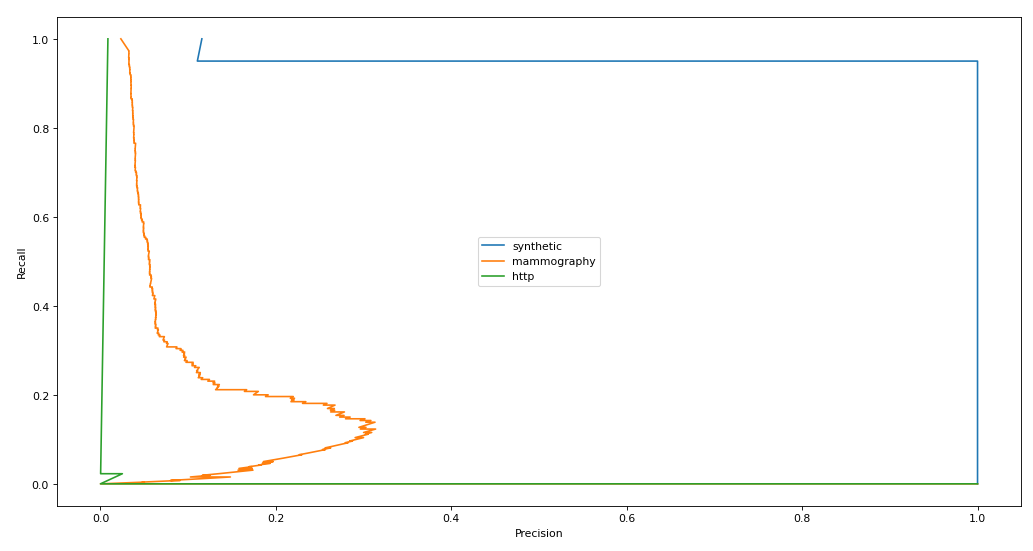
\includegraphics[width=\textwidth]{img/recall_precision_cof.png}
            \caption
            {Wykres recall od precision dla metody COF dla 3 zbiorów danych}
            \label{fig:cof}
        \end{figure}

        \begin{figure}[!htbp]
            \centering
            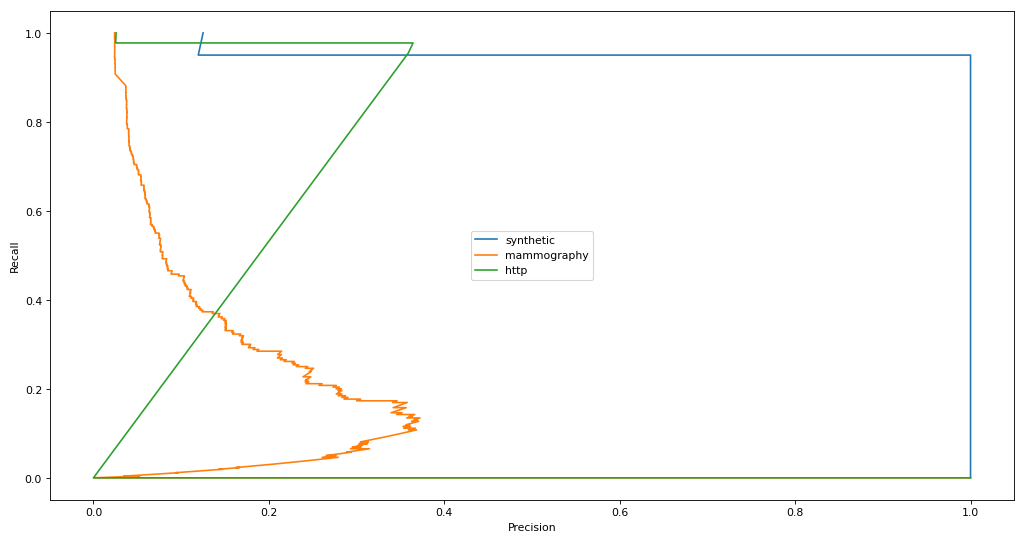
\includegraphics[width=\textwidth]{img/recall_precision_lof.png}
            \caption
            {Wykres recall od precision dla metody LOF dla 3 zbiorów danych}
            \label{fig:lof}
        \end{figure}
        \FloatBarrier
    }

    \section{Dyskusja i wnioski} {
        Na rysunkach \ref{fig:abod}, \ref{fig:cof} oraz \ref{fig:lof}
        widzimy krzywe precision-recall prezentujące jakość klasyfikacji
        wyjątków dla trzech różnych zbiorów danych. Jak widać dla zbioru
        ,,synthetic'' wszystkie trzy metody sprawdziły się niemal idealnie
        - precision równe 1 i recall ponad 0.9. Oznacza to, że właściwie
        wszystkie wyjątki zostały odnalezione. Wynika to z charakterystyki
        tego zbioru, który jest wygenerowany sztucznie, zawiera bardzo mało
        punktów a same wyjątki wyraźnie są oddzielone od pozostałych
        elementów. Nie ma tutaj istotnej różnicy między wynikami dla
        poszczególnych algorytmów, każdy sprawdził się doskonale.

        Zupełnie inaczej ma się sytuacja ze zbiorami rzeczywistymi:
        ,,mammography'' oraz ,,http''. Krzywa związana z tym pierwszym ma
        ciekawy kształt i generalnie oznacza raczej niskiej jakości
        klasyfikator. Widać tutaj wyraźnie, dla wszystkich trzech
        algorytmów, że wraz ze wzrostem wartości progu funkcji decyzyjnej
        rośnie precyzja, ale od razu znacząco maleje czułość. Za optymalny
        wynik można by uznać zarówno recall jak i precision mające wartości
        ok. 0.2. Jest to więc, jak już wspomniano wyżej, wynik niskiej
        jakości. Jako że jest to jednak zbiór rzeczywisty, nie wiadomo, czy
        uzyskanie wyniku lepszego jest w ogóle możliwe. Można powiedzieć,
        że spośród wszystkich trzech algorytmów najlepiej sprawdził się
        właśnie ABOD, ponieważ potrafi osiągnąć wyższą precyzję niż
        pozostałe, co widać na rysunku \ref{fig:abod} (pomarańczowa
        krzywa). Warto jeszcze wspomnieć o tym, że krzywa dla zbioru
        ,,mammography'' jest nietypowa, ponieważ ,,zawraca'' w pewnym
        momencie - nie udaje się osiągnąć dużych wartoći precyzji kosztem
        małej czułości. Może to oznaczać, że kilka punktów, które z dużym
        prawdopodobieństwem uznane są za wyjątki, wyjątkami nie są.

        Ostatni zbiór to ,,http''. Wyniki dla tego zbioru również są
        ciekawe, ponieważ widać, że do pewnego momentu (rysunki
        \ref{fig:lof} i \ref{fig:abod}) czułość klasyfikatora pozostaje
        bardzo duża przy rosnącej precyzji. Dochodzi jednak do momentu,
        kiedy obie miary spadają do zera i dopiero dla bardzo małych
        wartości czułości, precyzja rośnie od razu do maksimum. Zjawisko
        utrzymywania się wysokiej czułości dla coraz większej precyzji w
        ogóle nie wystąpiło dla metody COF, jest natomiast bardziej
        widoczne dla metody LOF, która osiągnęła tym samym najlepsze wyniki
        dla tego zbioru danych. Można to tłumaczyć obecnością jakiejś
        zbliżonej do siebie grupy punktów, stanowiących niemalże wszystkie
        wyjątki. Nie udaje się jednak rozpoznać tylko tych wyjątków, bez
        uwzględnienia dużej liczby wyników fałszywie pozytywnych (niska
        precyzja). Możliwe, że dla wszystkich algorytmów można by poprawić
        wyniki w tym zbiorze uwzględniając większą liczbę najbliższych
        sąsiadów.

        Podsumowując wszystkie algorytmy sprawowały się raczej podobnie.
        Nie wykazano, żeby algorytm ABOD działał znacząco lepiej niż LOF
        lub COF. Jego przewaga leży jednak w radzeniu sobie z bardzo dużą
        liczbą wymiarów, która nie wystąpiła w żadnym z analizowanych
        zbiorów danych.
    }

    \begin{thebibliography}{0}
        % @formatter:off
        \bibitem{pyod}{https://pyod.readthedocs.io/en/latest/}
        \bibitem{odds}{http://odds.cs.stonybrook.edu/}
        % @formatter:on
    \end{thebibliography}

\end{document}
